% Và như thường lệ, tôi sẽ trình bày một phương pháp đơn giản nhất trong các thuật toán Dimensionality Reduction dựa trên một mô hình tuyến tính. Phương pháp này có tên là \textit{Principal Component Analysis} (PCA), tức \textit{Phân tích thành phần chính}. Phương pháp này dựa trên quan sát rằng dữ liệu thường không phân bố ngẫu nhiên trong không gian mà thường phân bố gần các đường/mặt đặc biệt nào đó. PCA xem xét một trường hợp đặc biệt khi các mặt đặc biệt đó có dạng tuyến tính là các không gian con (subspace). 
  
% Trước khi đi vào chi tiết của PCA, chúng ta cùng điểm lại một chút về Đại số tuyến tính và Thống kê. 
 
 
% \section{Một chút toán}
 
 
% \subsection{Norm 2 của ma trận}
% Chúng ta vẫn thường nhắc nhiều đến \href{http://machinelearningcoban.com/math/#-norms-chuan}{norm cho vector} nhưng chưa thực sự làm việc nhiều với norm của ma trận (ngoài \href{http://machinelearningcoban.com/math/#chuan-cua-ma-tran}{Frobenius norm}). Trong mục này, chúng ta sẽ làm quen với 1 lớp các norm cho ma trận được định nghĩa dựa trên norm của vector. Lớp các norms này còn được gọi là \textit{Induced Norms}. 
 
% Giả sử hàm số $\|\mathbf{x}\|_{\alpha}$ là một norm bất kỳ của vector $\mathbf{x}$. Ứng với norm này, định nghĩa norm tương ứng cho ma trận $\mathbf{A}$: 
% \begin{equation} 
% \|\mathbf{A}\|_{\alpha} = \max_{\mathbf{x}} \frac{\|\mathbf{Ax}\|_{\alpha}}{\|\mathbf{x}\|_{\alpha}} 
% \end{equation} 
 
% chú ý rằng ma trận $\mathbf{A}$ có thể không vuông và số cột của nó bằng với số chiều của $\mathbf{x}$. Như vậy, bản thân việc tính toán norm của ma trận là việc giải một bài toán tối ưu. Chú ý rằng hàm tối ưu có cả tử số và mẫu số là các norm trên vectors. 
 
% Chúng ta sẽ quan tâm nhiều hơn tới norm 2. Norm 2 của ma trận được định nghĩa là: 
% \begin{equation} 
% \label{eqn:27_1}
% \|\mathbf{A}\|_2 = \max_{\mathbf{x}} \frac{\|\mathbf{Ax}\|_2}{\|\mathbf{x}\|_2}
% \end{equation} 
 
% Nhận thấy rằng nếu $\mathbf{x}$ là nghiệm của bài toán tối ưu \eqref{eqn:27_1} thì $k\mathbf{x}$ cũng là nghiệm với $k$ là một số thực khác không bất kỳ. Không mất tính tổng quát, ta có thể giả sử mẫu số bằng 1. Khi đó, bài toán tối ưu \eqref{eqn:27_1} có thể được viết dưới dạng: 
% \begin{equation} 
%     \label{eqn:27_2}
%     \|\mathbf{A}\|_2 = \max_{\|\mathbf{x}\|_2 = 1} \|\mathbf{Ax}\|_2
% \end{equation} 
% Nói cách khác, ta cần đi tìm $\mathbf{x}$ sao cho: 
% \begin{equation}
% \label{eqn:27_3} 
% \begin{aligned} 
% \mathbf{x} &= \text{argmax}_{\mathbf{x}} \|\mathbf{Ax}\|_2^2  \\\ 
% \text{thoả mãn: } & \|\mathbf{x}\|_2^2 = 1  
% \end{aligned} 
% \end{equation} 
% Ở đây, các norm 2 đã được bình phương lên để tránh dấu căn bậc hai. Bài toán \eqref{eqn:27_3} có thể được giải bằng \href{http://machinelearningcoban.com/2017/04/02/duality/# -- phuong-phap-nhan-tu-lagrange}{Phương pháp nhân tử Lagrange} vì ràng buộc là một phương trình. 
 
% Lagrangian của Bài toán \eqref{eqn:27_3} là: 
% \begin{equation} 
% \mathcal{L}(\mathbf{x}, \lambda) = \|\mathbf{Ax}\|_2^2 + \lambda (1 - \|\mathbf{x}\|_2^2) 
% \end{equation} 
 
% Nghiệm của bài toán \eqref{eqn:27_3} sẽ thoả mãn hệ phương trình: 
% \begin{eqnarray} 
%     \label{eqn:27_4}
%     \frac{\partial \mathcal{L}}{\partial \mathbf{x}} &=& 2\mathbf{A}^T\mathbf{Ax} - 2\lambda \mathbf{x} = \mathbf{0} \\\ 
%     \label{eqn:27_5}
%     \frac{\partial \mathcal{L}}{\partial \lambda} &=& 1 - \|\mathbf{x}\|_2^2 = 0  
% \end{eqnarray} 
 
% Từ \eqref{eqn:27_4} ta có: 
% \begin{equation} 
%     \label{eqn:27_6}
%     \mathbf{A}^T\mathbf{Ax} = \lambda\mathbf{x}  
% \end{equation} 
% Điều này suy ra rằng $\lambda$ là một trị riêng của $\mathbf{A}^T\mathbf{A}$ và $\mathbf{x}$ là 1 vector riêng ứng với trị riêng đó. Tiếp tục nhân hai vế của \eqref{eqn:27_6} với $\mathbf{x}^T$ vào bên trái, ta có: 
% \begin{equation} 
% \mathbf{x}^T\mathbf{A}^T\mathbf{Ax} = \lambda \mathbf{x}^T\mathbf{x} = \lambda 
% \end{equation} 
% Nhận thấy rằng vế trái chính là $\|\mathbf{Ax}\|_2^2$ chính là hàm mục tiêu trong \eqref{eqn:27_3}. Vậy hàm mục tiêu đạt giá trị lớn nhất khi $\lambda$ đạt giá trị lớn nhất. Nói cách khác, $\lambda$ chính là trị riêng lớn nhất của $\mathbf{A}^T\mathbf{A}$ hay chính là \href{http://machinelearningcoban.com/2017/06/07/svd/#-nguon-goc-ten-goi-singular-value-decomposition}{singular value} lớn nhất của ma trận $\mathbf{A}$. 
 
% Như vậy, norm 2 của một ma trận chính là singular value lớn nhất của ma trận đó. Và nghiệm của bài toán \eqref{eqn:27_3} chính một là \textit{right-singular vector} ứng với singular value đó. 
 
% Với lý luận tương tự, chúng ta có thể suy ra rằng bài toán: 
% \begin{equation} 
%     \min_{\|\mathbf{x}\|_2 =1} \mathbf{x}^T\mathbf{A}^T\mathbf{A}\mathbf{x} 
% \end{equation} 
 
% có nghiệm là vector riêng ứng với trị riêng nhỏ nhất của $\mathbf{A}^T\mathbf{A}$. Khi đó, hàm số đạt giá trị nhỏ nhất bằng chính trị riêng nhỏ nhất này. 
 
 
 
 
 
% \subsection{Biễu diễn vector trong các hệ cơ sở khác nhau}
 
% Trong không gian $D$ chiều , toạ độ của mỗi điểm được xác định dựa trên một hệ toạ độ nào đó. Ở các hệ toạ độ khác nhau, hiển nhiên là toạ độ của mỗi điểm cũng khác nhau. 
 
% Tập hợp các vector $\mathbf{e}_1, \dots, \mathbf{e}_D$ mà mỗi vector $\mathbf{e}_d$ có đúng 1 phần tử khác 0 ở thành phần thứ $d$ và phần tử đó bằng 1, được gọi là hệ cơ sở đơn vị (hoặc hệ đơn vị) trong không gian $D$ chiều. Nếu xếp các vector $\mathbf{e}_d, d = 1, 2, \dots, D$ theo đúng thứ tự đó, ta sẽ được ma trận đơn vị $D$ chiều. 
 
% Mỗi vector cột $\mathbf{x} = [x_1, x_2, \dots, x_D] \in \mathbb{R}^D$, biểu diễn của nó trong hệ đơn vị là: 
 
% \begin{equation} 
%     \mathbf{x} = x_1 \mathbf{e}_1 + x_2 \mathbf{e}_2 + \dots + x_D\mathbf{e}_D 
% \end{equation} 
 
% Giả sử có một hệ cơ sở khác $\mathbf{u}_1, \mathbf{u}_2, \dots, \mathbf{u}_D$ (các vector này độc lập tuyến tính), vậy thì biểu diễn của vector $\mathbf{x}$ trong hệ cơ sở mới này có dạng: 
 
% \begin{equation} 
%     \mathbf{x} = y_1 \mathbf{u}_1 + y_2 \mathbf{u}_2 + \dots + y_D\mathbf{u}_D  = \bU\mathbf{y} 
% \end{equation} 
 
% $\bU$ là ma trận mà cột thứ $d$ của nó chính là vector $\mathbf{u}_d$. Lúc này, vector $\mathbf{y}$ chính là biểu diễn của $\mathbf{x}$ trong hệ cơ sở mới. Bộ các số $y_d, d = 1, 2, \dots, D$ là duy nhất vì $\mathbf{y}$ có thể tính được bằng: 
% \begin{equation} 
%     \label{eqn:27_7}
%     \mathbf{y} = \bU^{-1} \mathbf{x} 
% \end{equation} 
% với chú ý rằng $\bU$ là ma trận khả nghịch vì các cột của nó độc lập tuyến tính. 
 
% Trong các ma trận đóng vai trò như hệ cơ sở $\bU$, \href{http://machinelearningcoban.com/2017/06/07/svd/#-he-truc-giao-va-truc-chuan}{các ma trận trực giao}, tức $\bU^T\bU = \mathbf{I}$, được quan tâm nhiều hơn vì nghịch đảo của chúng chính là chuyển vị của chúng: 
% \begin{equation} 
%     \bU^{-1} = \bU^T 
% \end{equation} 
% Khi đó, $\mathbf{y}$ trong \eqref{eqn:27_7} có thể được tính một cách nhanh chóng: 
 
% \begin{equation} 
%     \mathbf{y} = \bU^{T} \mathbf{x} 
% \end{equation} 
% từ đó suy ra: $y_i = \mathbf{x}^T \mathbf{u}_i = \mathbf{u}_i^T\mathbf{x}, i= 1, 2, \dots, D$. 
 
% Có thể nhận thấy rằng vector $\mathbf{0}$ được biểu diễn như nhau trong mọi hệ cơ sở. 
% Hình 1 dưới đây là 1 ví dụ về việc chuyển hệ cơ sở: 
 
% % <hr> 
% % <div> 
% % <table width = "100%" style = "border: 0px solid white"> 
 
% %     <tr > 
% %         <td width="40%" style = "border: 0px solid white" align = "center"> 
% %         <img style="display:block;" width = "100%" src = "/assets/27_pca/changebasis.png"> 
% %          </td> 
% %         <td width="40%" style = "border: 0px solid white" align = "justify"> 
% %         Hình 1: Chuyển đổi toạ độ trong các hệ cơ sở khác nhau. 
 
% %         </td> 
% %     </tr> 
% % </table> 
% % </div> 
% % <hr> 
% \begin{figure}[t]
%     % caption on side     
%     \floatbox[{\capbeside\thisfloatsetup{capbesideposition={right,top},capbesidewidth=6cm}}]{figure}[\FBwidth]
%     {\caption{ 
%     Chuyển đổi toạ độ trong các hệ cơ sở khác nhau.
%     }
%     \label{fig:27_1}}
%     { % figure here
%     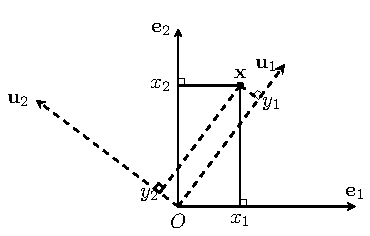
\includegraphics[width=.5\textwidth]{Chapters/07_DimemsionalityReduction/27_pca/latex/changebasis.pdf}
%     }
% \end{figure}

 
% Việc chuyển đổi hệ cơ sở sử dụng ma trận trực giao có thể được coi như một phép xoay trục toạ độ. Nhìn theo một cách khác, đây cũng chính là một phép xoay vector dữ liệu theo chiều ngược lại. 
% \subsection{Trace}
 
% Hàm số trace xác định trên tập các ma trận vuông được sử dụng rất nhiều trong tối ưu vì những tính chất đẹp của nó. Hàm trace trả về tổng các phần tử trên đường chéo của một ma trận vuông. 
 
% Các tính chất quan trọng của hàm trace, với giả sử rằng các ma trận trong hàm trace là vuông và các phép nhân ma trận thực hiện được: 
% \begin{itemize}
%     \item $\text{trace}(\mathbf{A}) = \text{trace}(\mathbf{A}^T)$ 
     
%     \item $\text{trace}(k\mathbf{A}) = k\text{trace}(\mathbf{A})$ với $k$ là một số bất kỳ. 
     
%     \item $\text{trace}(\mathbf{AB}) = \text{trace}(\mathbf{BA})$ 
     
%     \item $\|\mathbf{A}\|_F^2 = \text{trace}(\mathbf{A}^T\mathbf{A}) = \text{trace}(\mathbf{A}\mathbf{A}^T)$ với $\mathbf{A}$ là ma trận bất kỳ, có thể không vuông. 
     
%     \item $\text{trace}(\mathbf{A}) = \sum_{i = 1}^D \lambda_i $ với $\mathbf{A}$ là một ma trận vuông và $\lambda_i, i = 1, 2, \dots, N$ là toàn bộ các trị riêng của nó, có thể phức hoặc lặp. Việc chứng minh tính chất này có thể được dựa trên ma trận đặc trưng của $\mathbf{A}$ và định lý Viète. Tôi xin được bỏ qua. 
% \end{itemize}
 
 
% \subsection{Kỳ vọng và ma trận hiệp phương sai}
 
% \subsubsection{Dữ liệu một chiều}
 
% Cho $N$ giá trị $x_1, x_2, \dots, x_N$. \textit{Kỳ vọng} và \textit{phương sai} của bộ dữ liệu này được định nghĩa là: 
 
% \begin{eqnarray} 
%     \bar{x} &=& \frac{1}{N}\sum_{n=1}^N x_n = \frac{1}{N}\mathbf{X1}\\\ 
%     \sigma^2 &=& \frac{1}{N} \sum_{n=1}^N (x_n - \bar{x})^2 
% \end{eqnarray} 
% với $\mathbf{1} \in \mathbb{R}^N$ là vector cột chứa toàn phần tử 1. 
% Kỳ vọng đơn giản là trung bình cộng của toàn bộ các giá trị. Phương sai là trung bình cộng của bình phương khoảng cách từ mỗi điểm tới kỳ vọng. Phương sai càng nhỏ thì các điểm dữ liệu càng gần với kỳ vọng, tức các điểm dữ liệu càng giống nhau. Phương sai càng lớn thì ta nói dữ liệu càng có tính phân tán. Ví dụ về kỳ vọng và phương sai của dữ liệu một chiều có thể được thấy trong Hình 2a). 
 
% Căn bậc hai của phương sai, $\sigma$ còn được gọi là độ lệch chuẩn (standard deviation) của dữ liệu. 
 
 
% \subsubsection{Dữ liệu nhiều chiều}
 
% Cho $N$ điểm dữ liệu được biểu diễn bởi các vector cột $\mathbf{x}_1, \dots, \mathbf{x}_N$, khi đó, \textit{vector kỳ vọng} và \textit{ma trận hiệp phương sai} của toàn bộ dữ liệu được định nghĩa là: 
 
% \begin{eqnarray} 
%     \bar{\mathbf{x}} &=& \frac{1}{N} \sum_{n=1}^N \mathbf{x}_n \\\ 
%     \mathbf{S} &=&  \frac{1}{N}\sum_{n=1}^N (\mathbf{x}_n - \bar{\mathbf{x}})(\mathbf{x}_n - \bar{\mathbf{x}})^T = \frac{1}{N}\what{\bX}\what{\bX}^T 
% \end{eqnarray} 
% Trong đó $\what{\bX}$ được tạo bằng cách trừ mỗi cột của $\bX$ đi $\bar{\mathbf{x}}$: 
% \begin{equation} 
%     \hat{\mathbf{x}}_n = \mathbf{x}_n - \bar{\mathbf{x}} 
% \end{equation} 
 
% Các công thức này khá tương đồng với các công thức cho dữ liệu 1 chiều phía trên. Có một vài điểm lưu ý: 
% \begin{itemize}
%     \item Ma trận hiệp phương sai là một ma trận đối xứng, hơn nữa, nó là một ma trận \href{https://machinelearningcoban.com/2017/03/12/convexity/#positive-semidefinite}{nửa xác định dương}. 
     
%     \item Mọi phần tử trên đường chéo của ma trận hiệp phương sai là các số không âm. Chúng cũng chính là phương sai của từng chiều của dữ liệu. 
     
%     \item Các phần tử ngoài đường chéo $s_{ij}, i \neq j$ thể hiện sự tương quan giữa thành phần thứ $i$ và thứ $j$ của dữ liệu, còn được gọi là hiệp phương sai. Giá trị này có thể dương, âm hoặc bằng 0. Khi nó bằng 0, ta nói rằng hai thành phần $i, j$ trong dữ liệu là không tương quan (uncorrelated). 
     
%     \item Nếu ma trận hiệp phương sai là ma trận đường chéo, ta có dữ liệu hoàn toàn không tương quan giữa các chiều. 
% \end{itemize}
 
% Ví dụ về dữ liệu không tương quan và tương quan được cho trong Hình 2bc). 
% % <hr> 
% % <div> 
% % <table width = "100%" style = "border: 0px solid white"> 
% %     <tr > 
% %         <td width="40%" style = "border: 0px solid white" align = "center"> 
% %         <img style="display:block;" width = "100%" src = "/assets/27_pca/var_1d.png"> 
% %          <br> 
% %         a) 
% %          </td> 
% %          <td width="40%" style = "border: 0px solid white" align = "center"> 
% %          <img style="display:block;" width = "100%" src = "/assets/27_pca/pca_diagvar.png"> 
% %           <br> 
% %          b) 
% %           </td> 
% %     </tr> 
 
% %     <tr > 
% %         <td width="40%" style = "border: 0px solid white" align = "center"> 
% %         <img style="display:block;" width = "100%" src = "/assets/27_pca/pca_var0.png"> 
% %          <br> 
% %         c) 
% %          </td> 
% %          <td width="40%" style = "border: 0px solid white" align = "justify"> 
% %         Hình 2: Ví dụ về kỳ vọng và phương sai. a) Trong không gian 1 chiều. b) Không gian 2 chiều mà hai chiều không tương quan. Trong trường hợp này, ma trận hiệp phương sai là ma trận đường chéo với hai phần tử trên đường chéo  là $\sigma_1, \sigma_2$, đây cũng chính là hai trị riêng của ma trận hiệp phương sai và là phương sai của mỗi chiều dữ liệu. c) Dữ liệu trong không gian hai chiều có tương quan. Theo mỗi chiều, ta có thể tính được kỳ vọng và phương sai. Phương sai càng lớn thì dữ liệu trong chiều đó càng phân tán. Trong ví dụ này, dữ liệu theo chiều thứ hai phân tán nhiều hơn so so với chiều thứ nhất. 
% %           </td> 
% %     </tr> 
% % </table> 
% % </div> 
% % <hr> 
 
% %%%%%%% Three subfigures with bottom caption%%%%%%%%%%%%%%
%  \begin{figure}[t]
%      \begin{subfigure}{0.329\textwidth}
%      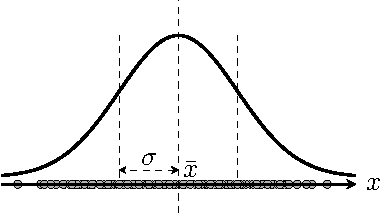
\includegraphics[width=0.99\linewidth]{Chapters/07_DimemsionalityReduction/27_pca/latex/var_1d.pdf}
%      \caption{}
%      % \label{fig:subim1}
%      \end{subfigure}
%      \begin{subfigure}{0.329\textwidth}
%      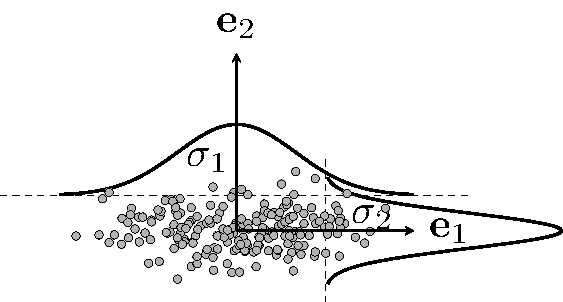
\includegraphics[width=0.99\linewidth]{Chapters/07_DimemsionalityReduction/27_pca/latex/pca_diagvar.pdf}
%      \caption{}
%      % \label{fig:subim2}
%      \end{subfigure}
%      \begin{subfigure}{0.329\textwidth}
%      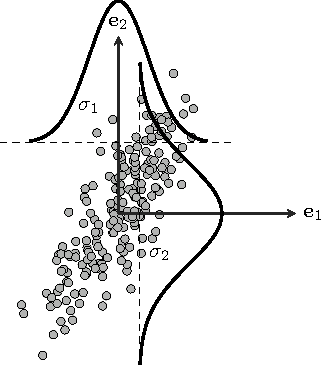
\includegraphics[width=0.99\linewidth]{Chapters/07_DimemsionalityReduction/27_pca/latex/pca_var0.pdf}
%      \caption{}
%      % \label{fig:subim2}
%      \end{subfigure}
%      \caption{
%      Ví dụ về kỳ vọng và phương sai. a) Trong không gian 1 chiều. b) Không gian 2 chiều mà hai chiều không tương quan. Trong trường hợp này, ma trận hiệp phương sai là ma trận đường chéo với hai phần tử trên đường chéo  là $\sigma_1, \sigma_2$, đây cũng chính là hai trị riêng của ma trận hiệp phương sai và là phương sai của mỗi chiều dữ liệu. c) Dữ liệu trong không gian hai chiều có tương quan. Theo mỗi chiều, ta có thể tính được kỳ vọng và phương sai. Phương sai càng lớn thì dữ liệu trong chiều đó càng phân tán. Trong ví dụ này, dữ liệu theo chiều thứ hai phân tán nhiều hơn so so với chiều thứ nhất. 
%      }
%      \label{fig:27_2}
%  \end{figure}
